\chapter{Running a Mapreduce program with 1-node}
\par In this section we will be Running a Mapreduce program in a single node cluster.
%Intro\footnotemark\\
\begin{spacing}{1.2}
%note en bas de page
\section{Preparing files}

\par First, we gotta make sure that our node is live.
\\
\begin{figure}[!htb] 
\begin{center} 
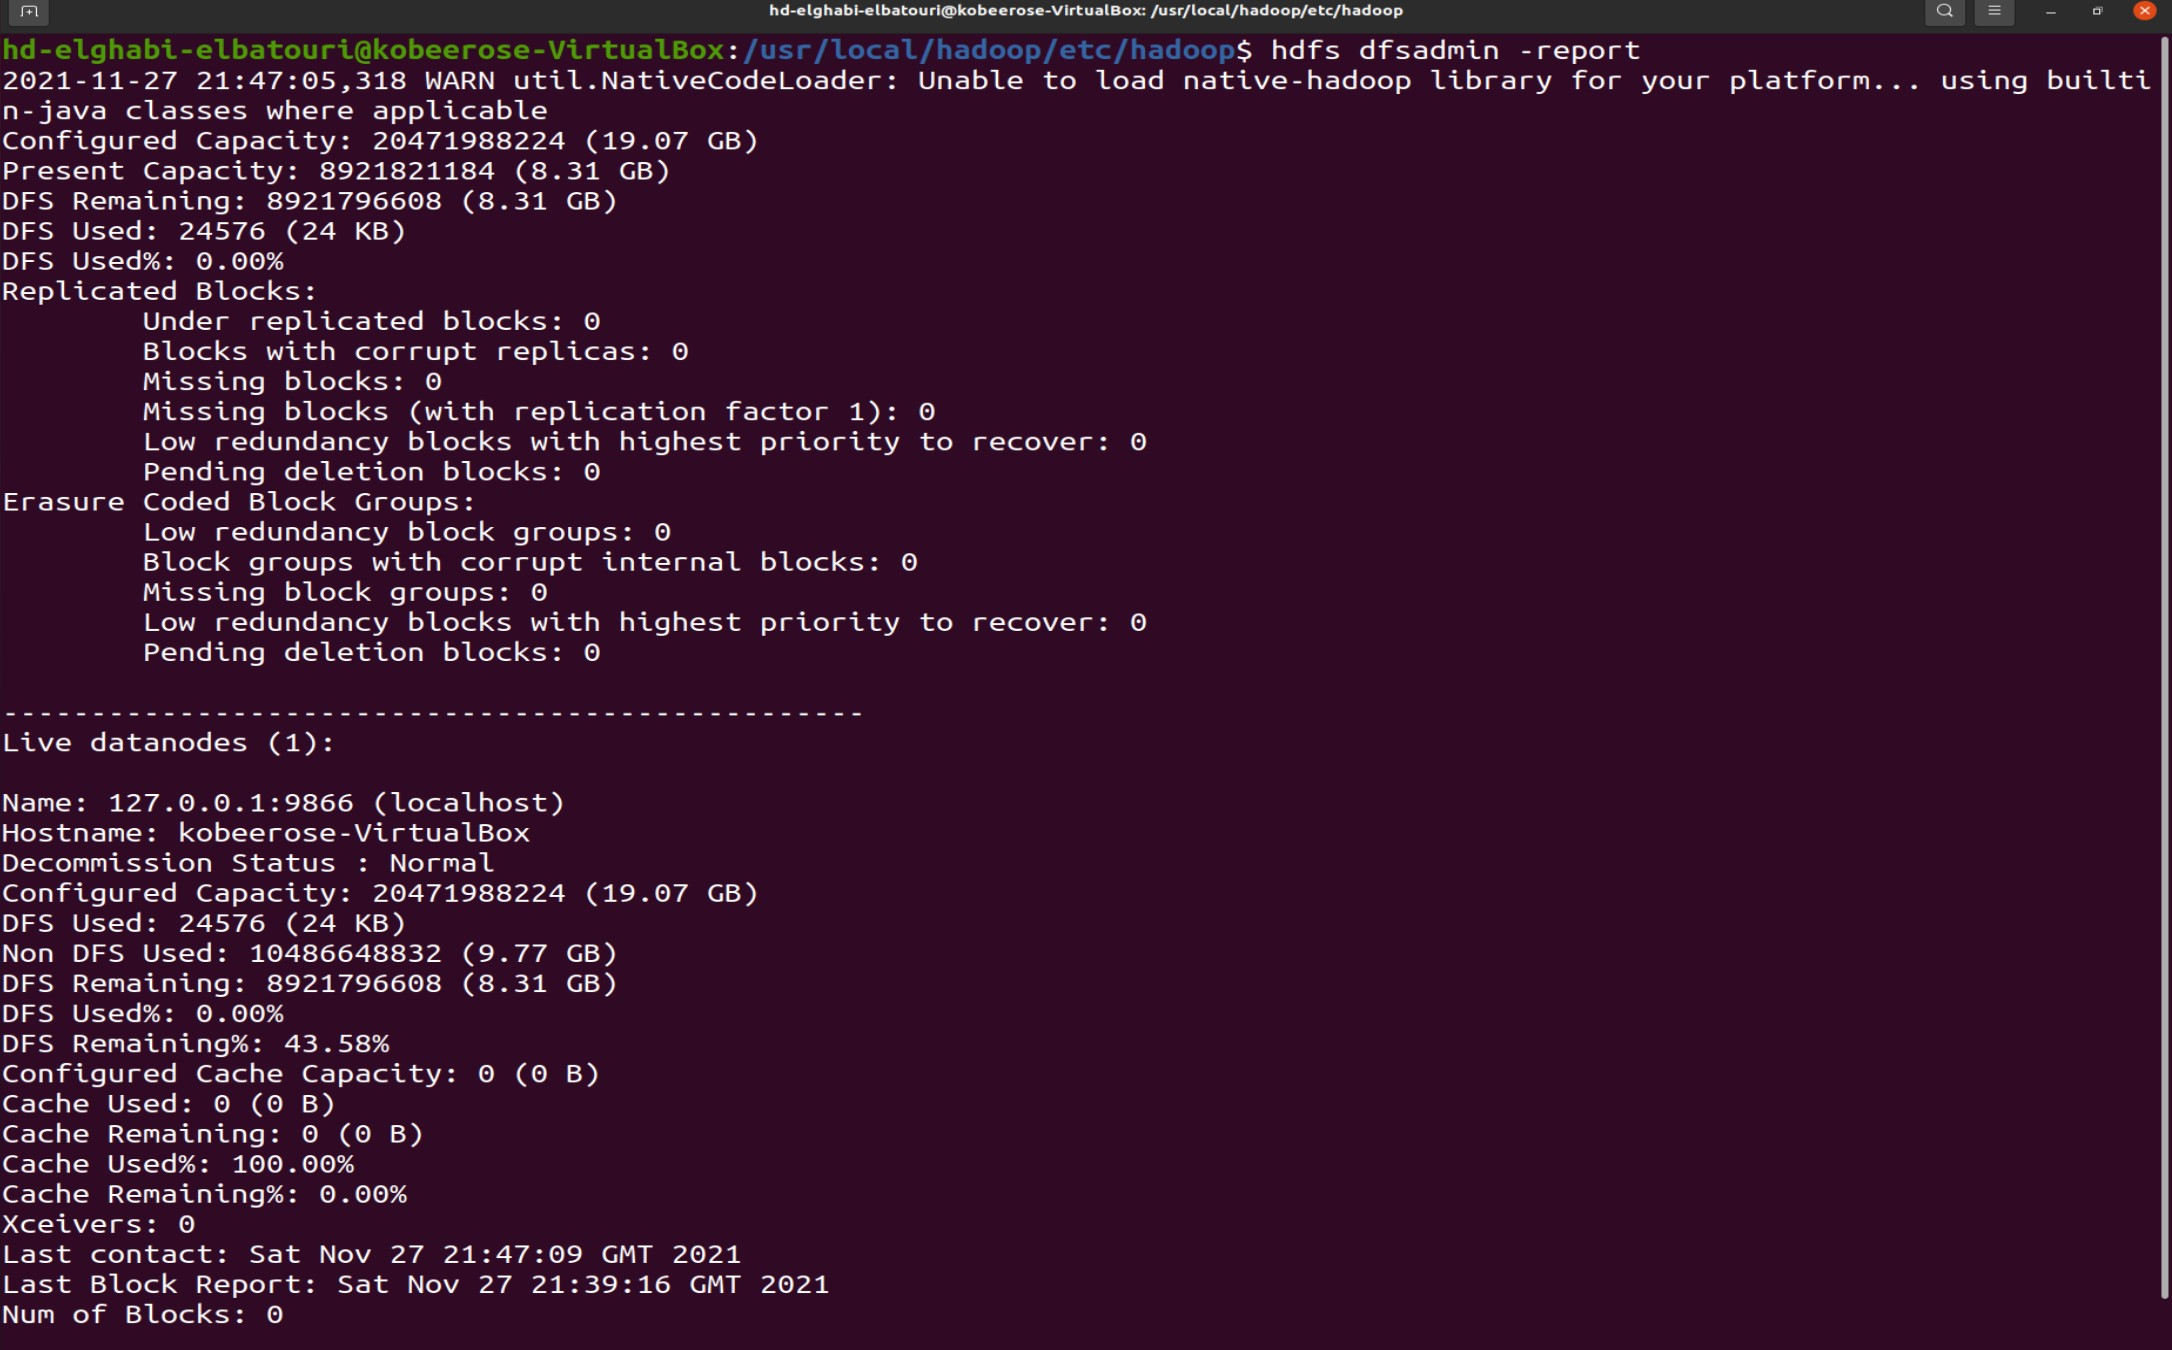
\includegraphics[width=1\linewidth]{Big_Data/Hadoop/1-Node Map_Reduce/HDFS Repport} 
\end{center} 
\caption{HDFS Repport} 
\end{figure} 
\FloatBarrier



\par Unzip the java code archive and create new directory.
\\
\begin{figure}[!htb] 
\begin{center} 
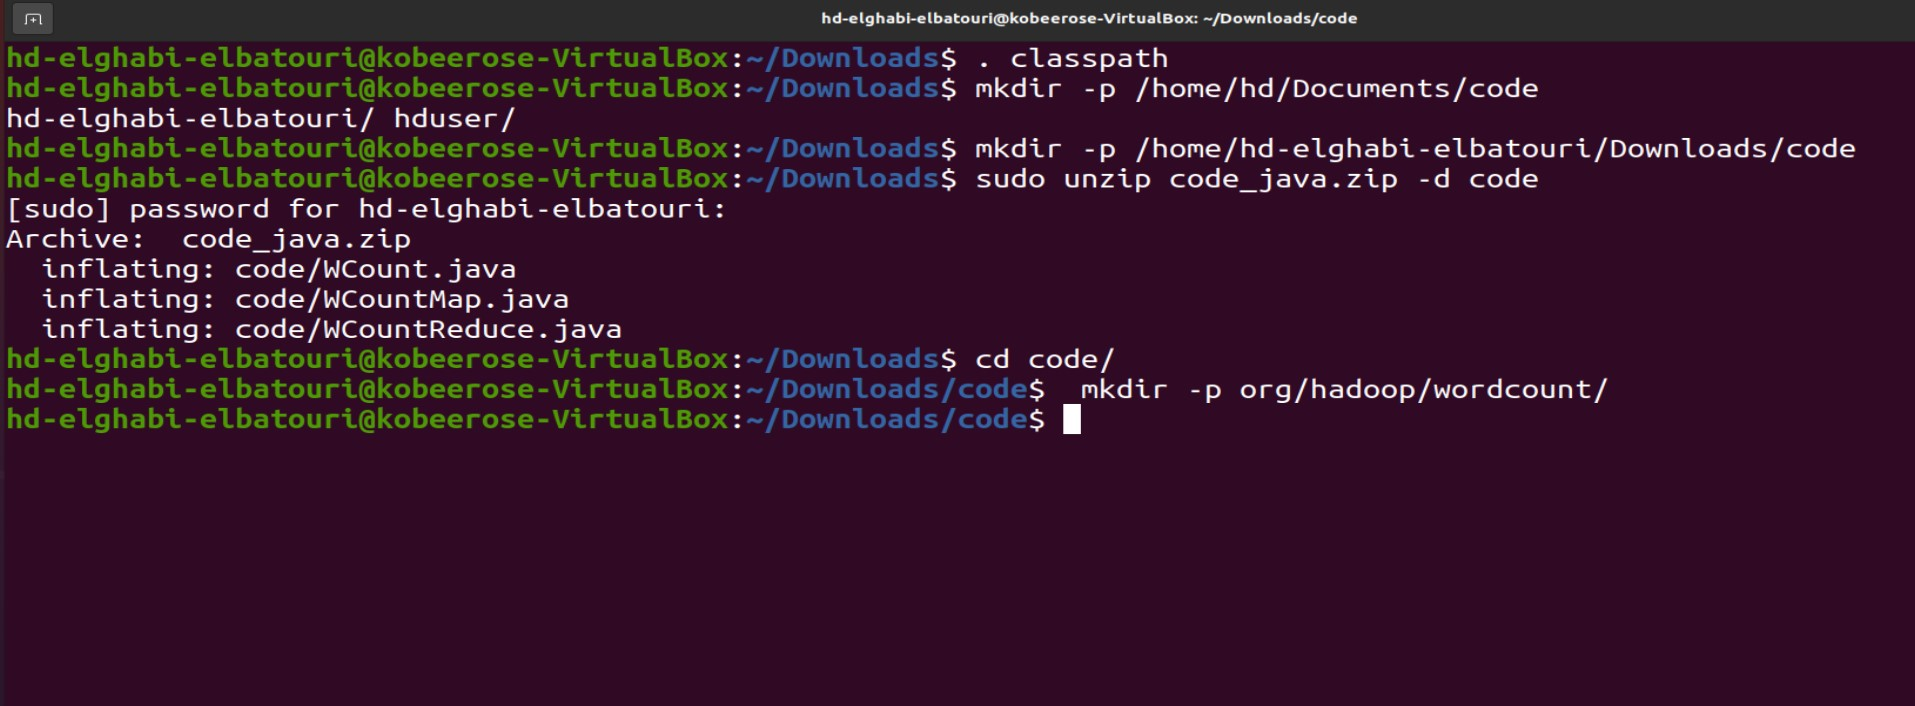
\includegraphics[width=1\linewidth]{Big_Data/Hadoop/1-Node Map_Reduce/Exporting jars} 
\end{center} 
\caption{Exporting jars} 
\end{figure} 
\FloatBarrier

\section{Working with jars}

\par Compile the java classes "Wcount.java, WcountMap.java and WcountReduce.ja
\\
\begin{figure}[!htb] 
\begin{center} 
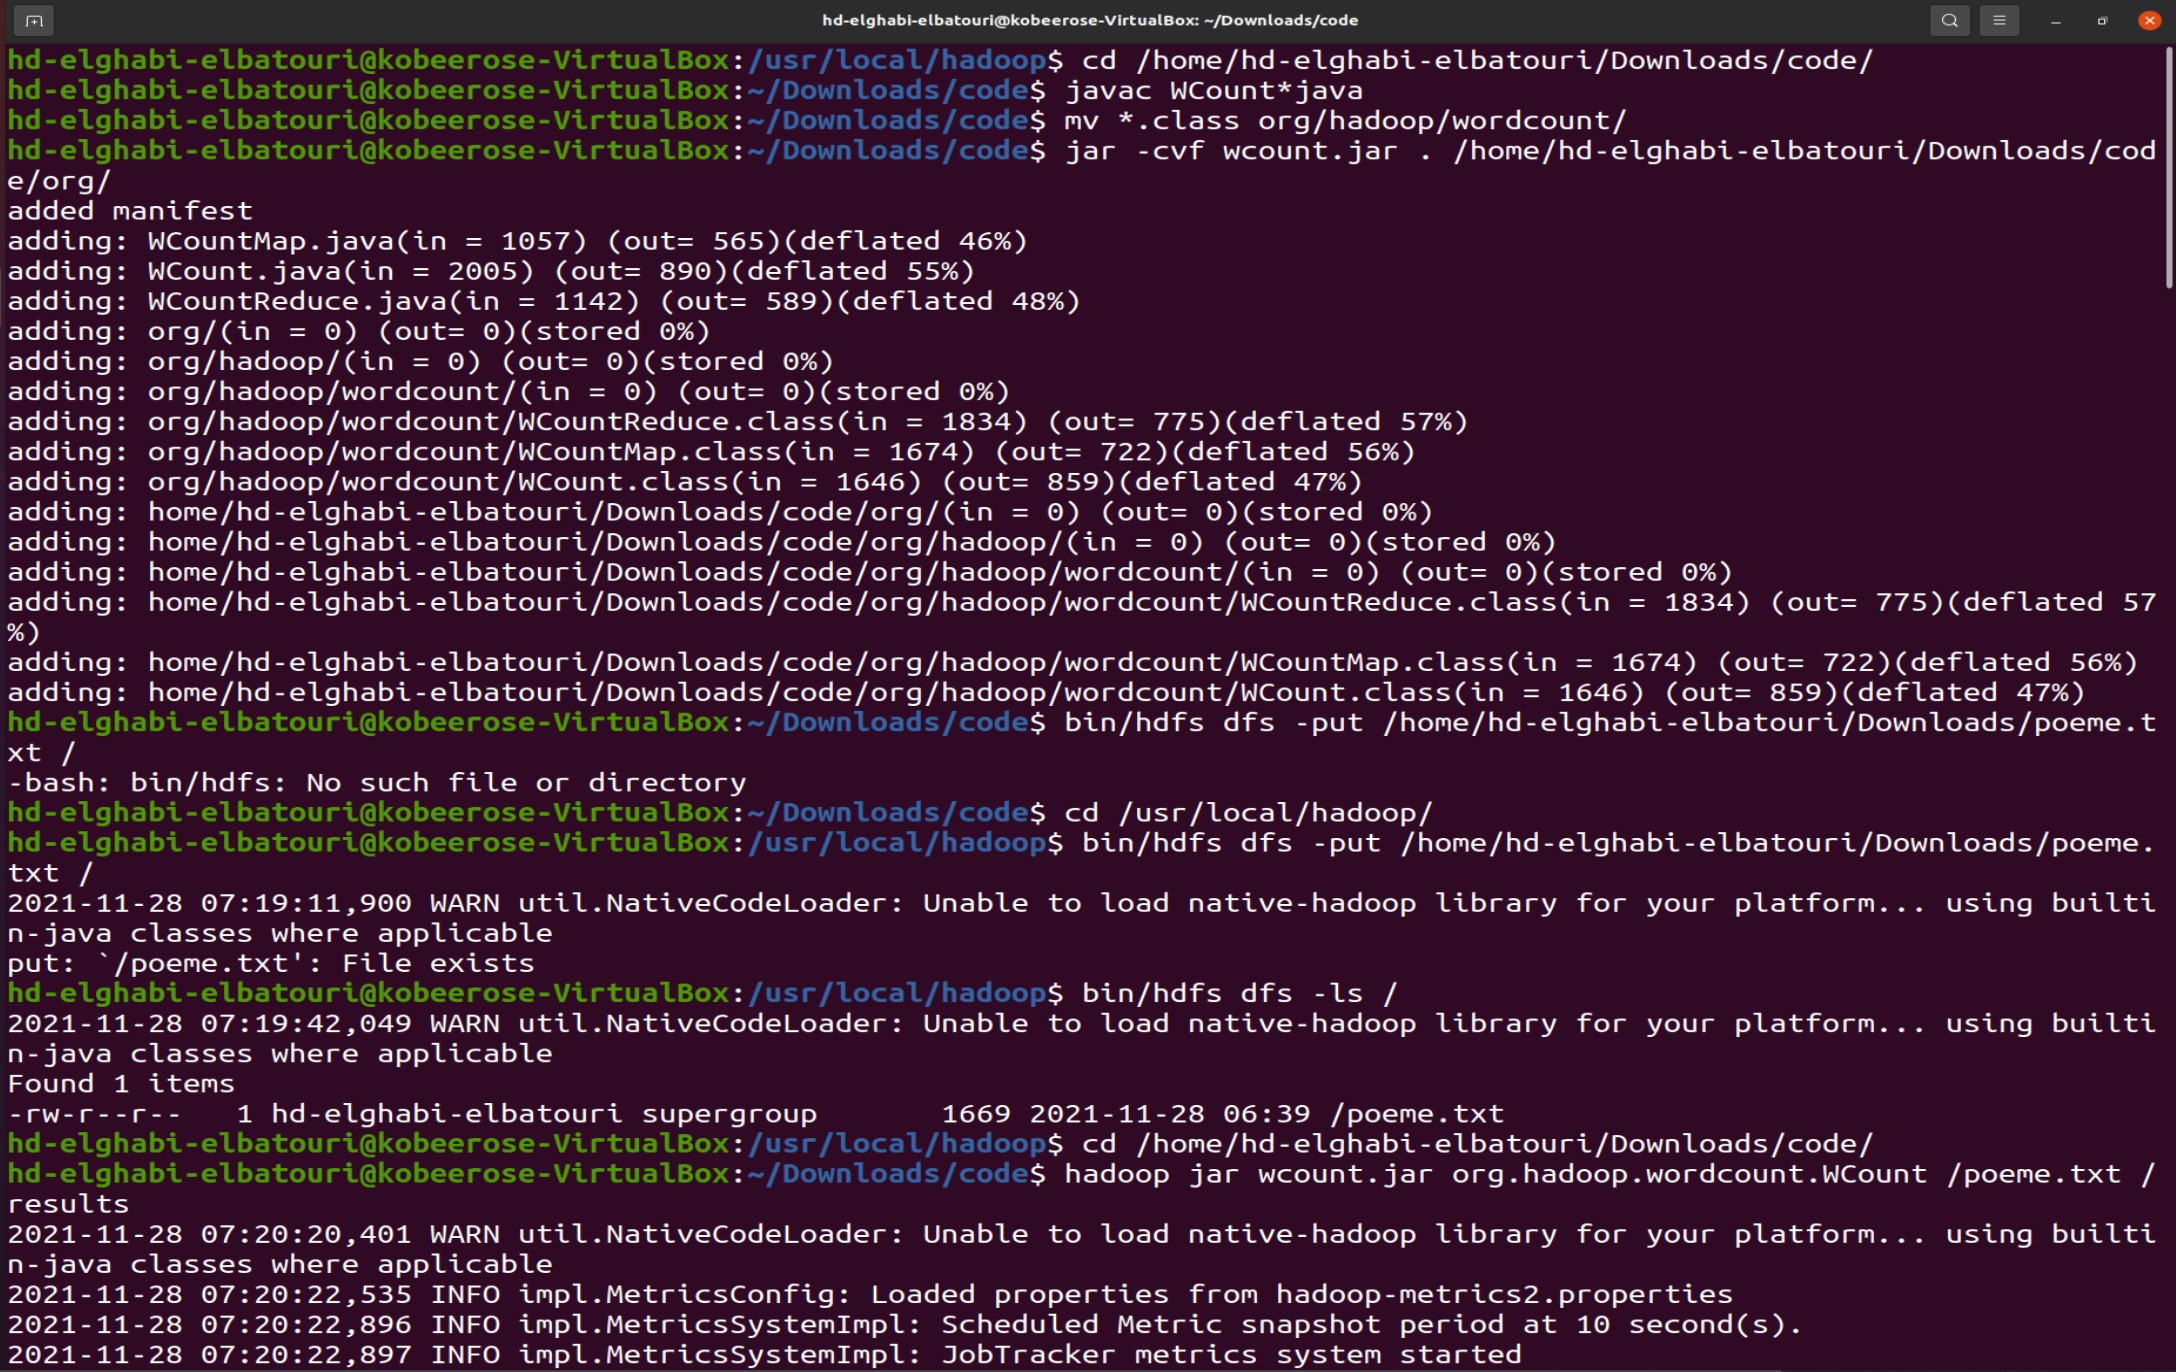
\includegraphics[width=1\linewidth]{Big_Data/Hadoop/1-Node Map_Reduce/Compiling jars} 
\end{center} 
\caption{Compiling jars} 
\end{figure} 
\FloatBarrier

\section{Executing Word Count}

\par Running Word Count algorithm on poeme.txt file.
\\
\begin{figure}[!htb] 
\begin{center} 
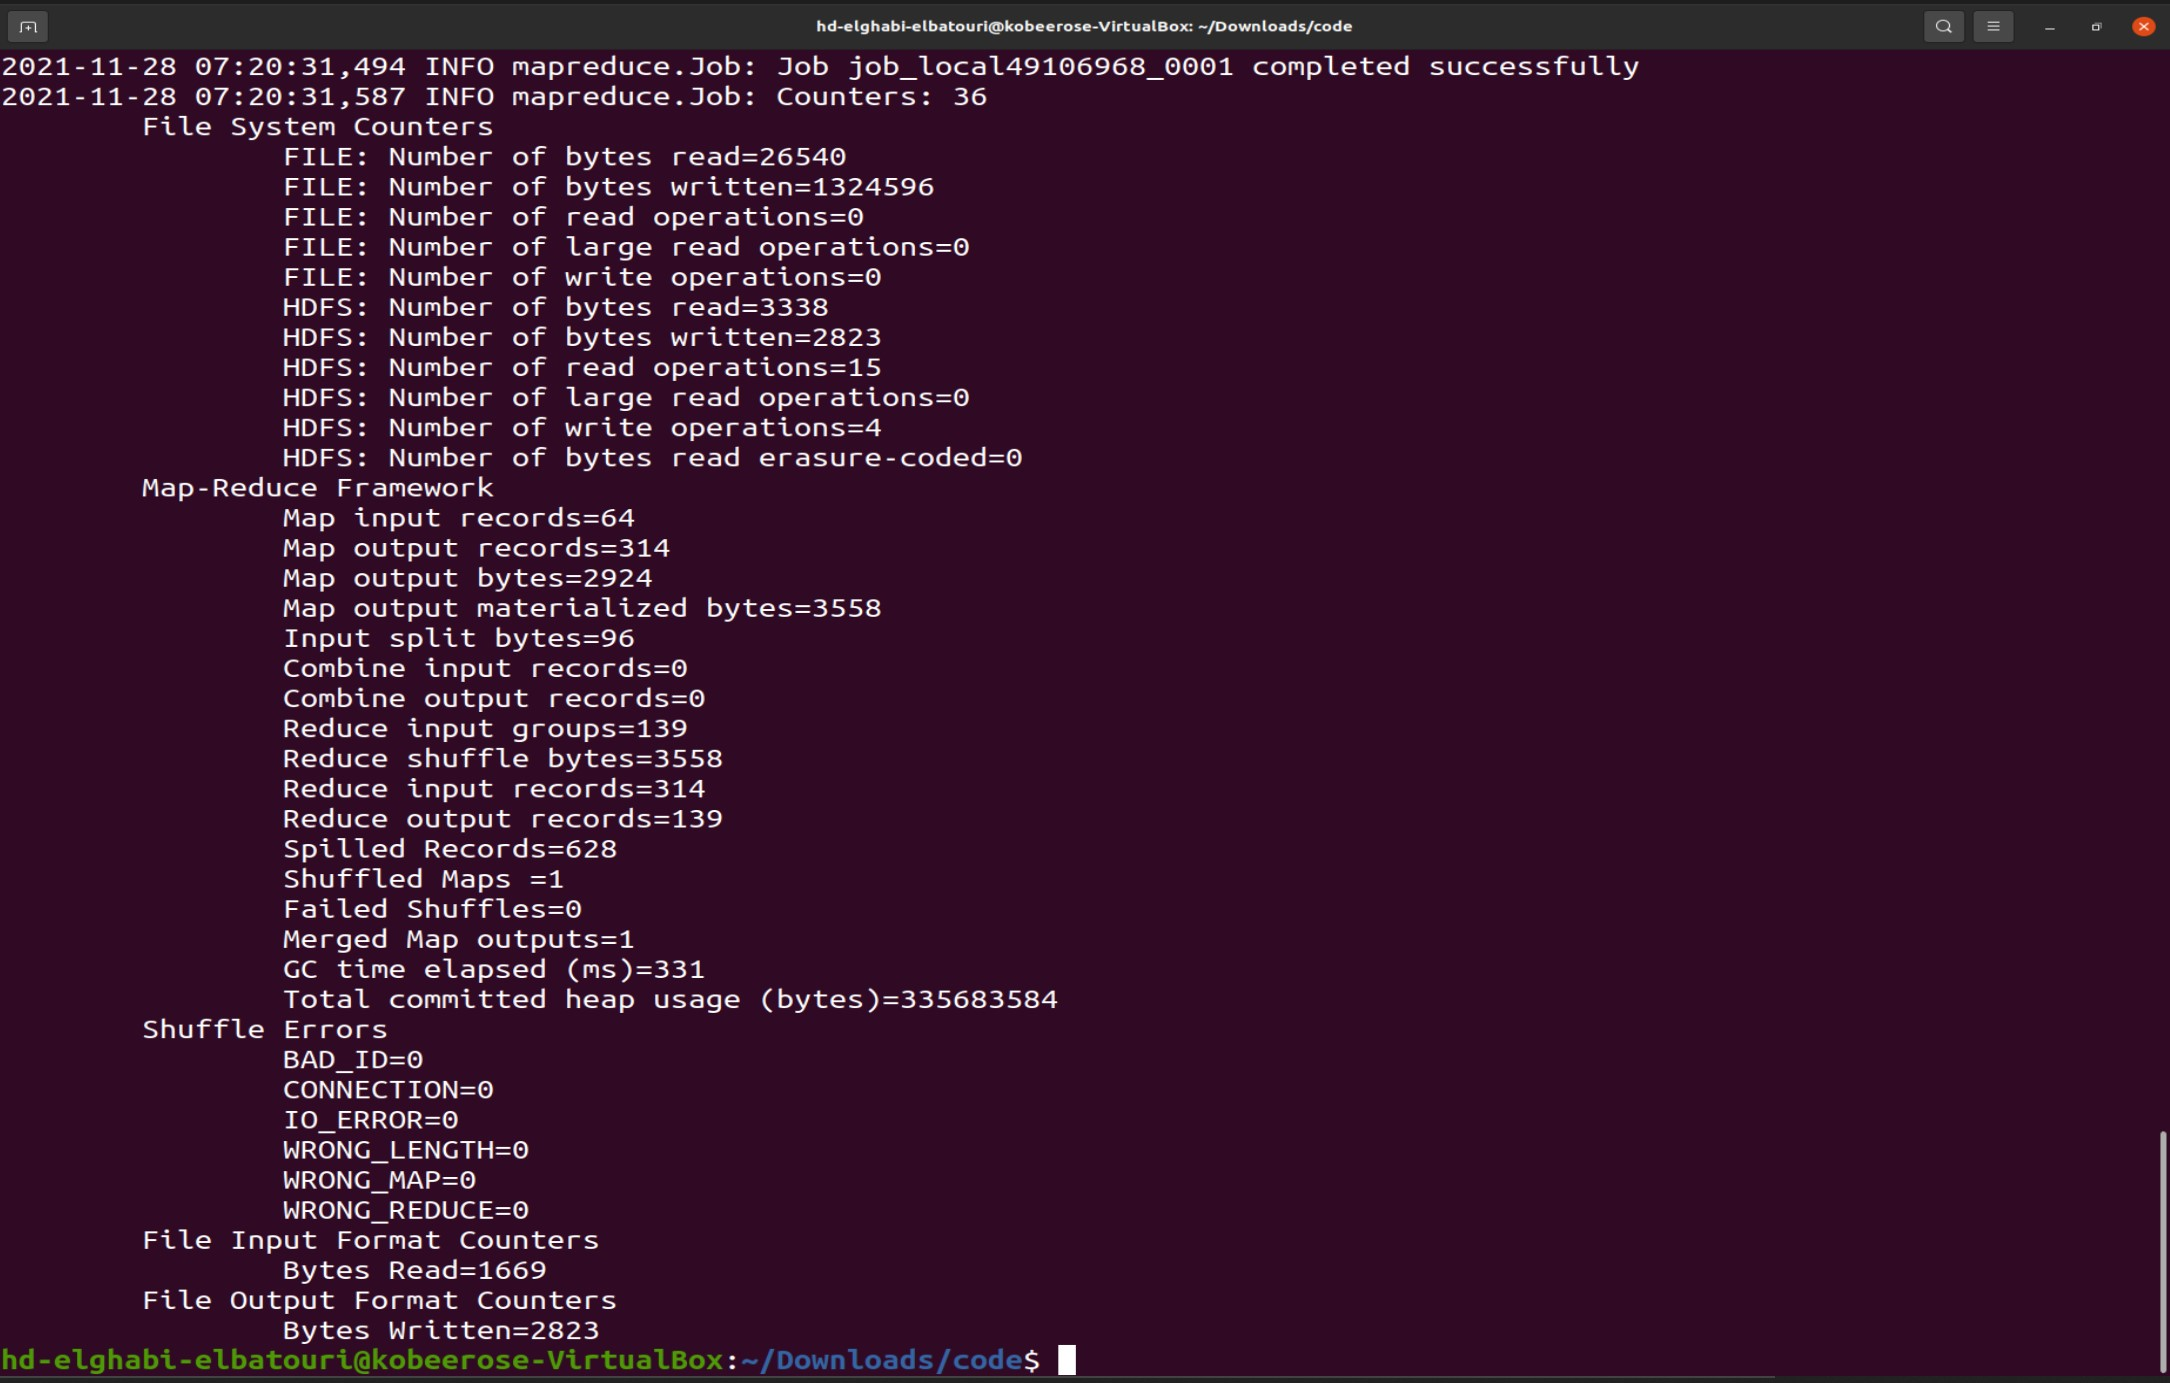
\includegraphics[width=1\linewidth]{Big_Data/Hadoop/1-Node Map_Reduce/running wordcount} 
\end{center} 
\caption{running wordcount} 
\end{figure} 
\FloatBarrier

\par Here is the result given by the algorithm.
\\
\begin{figure}[!htb] 
\begin{center} 
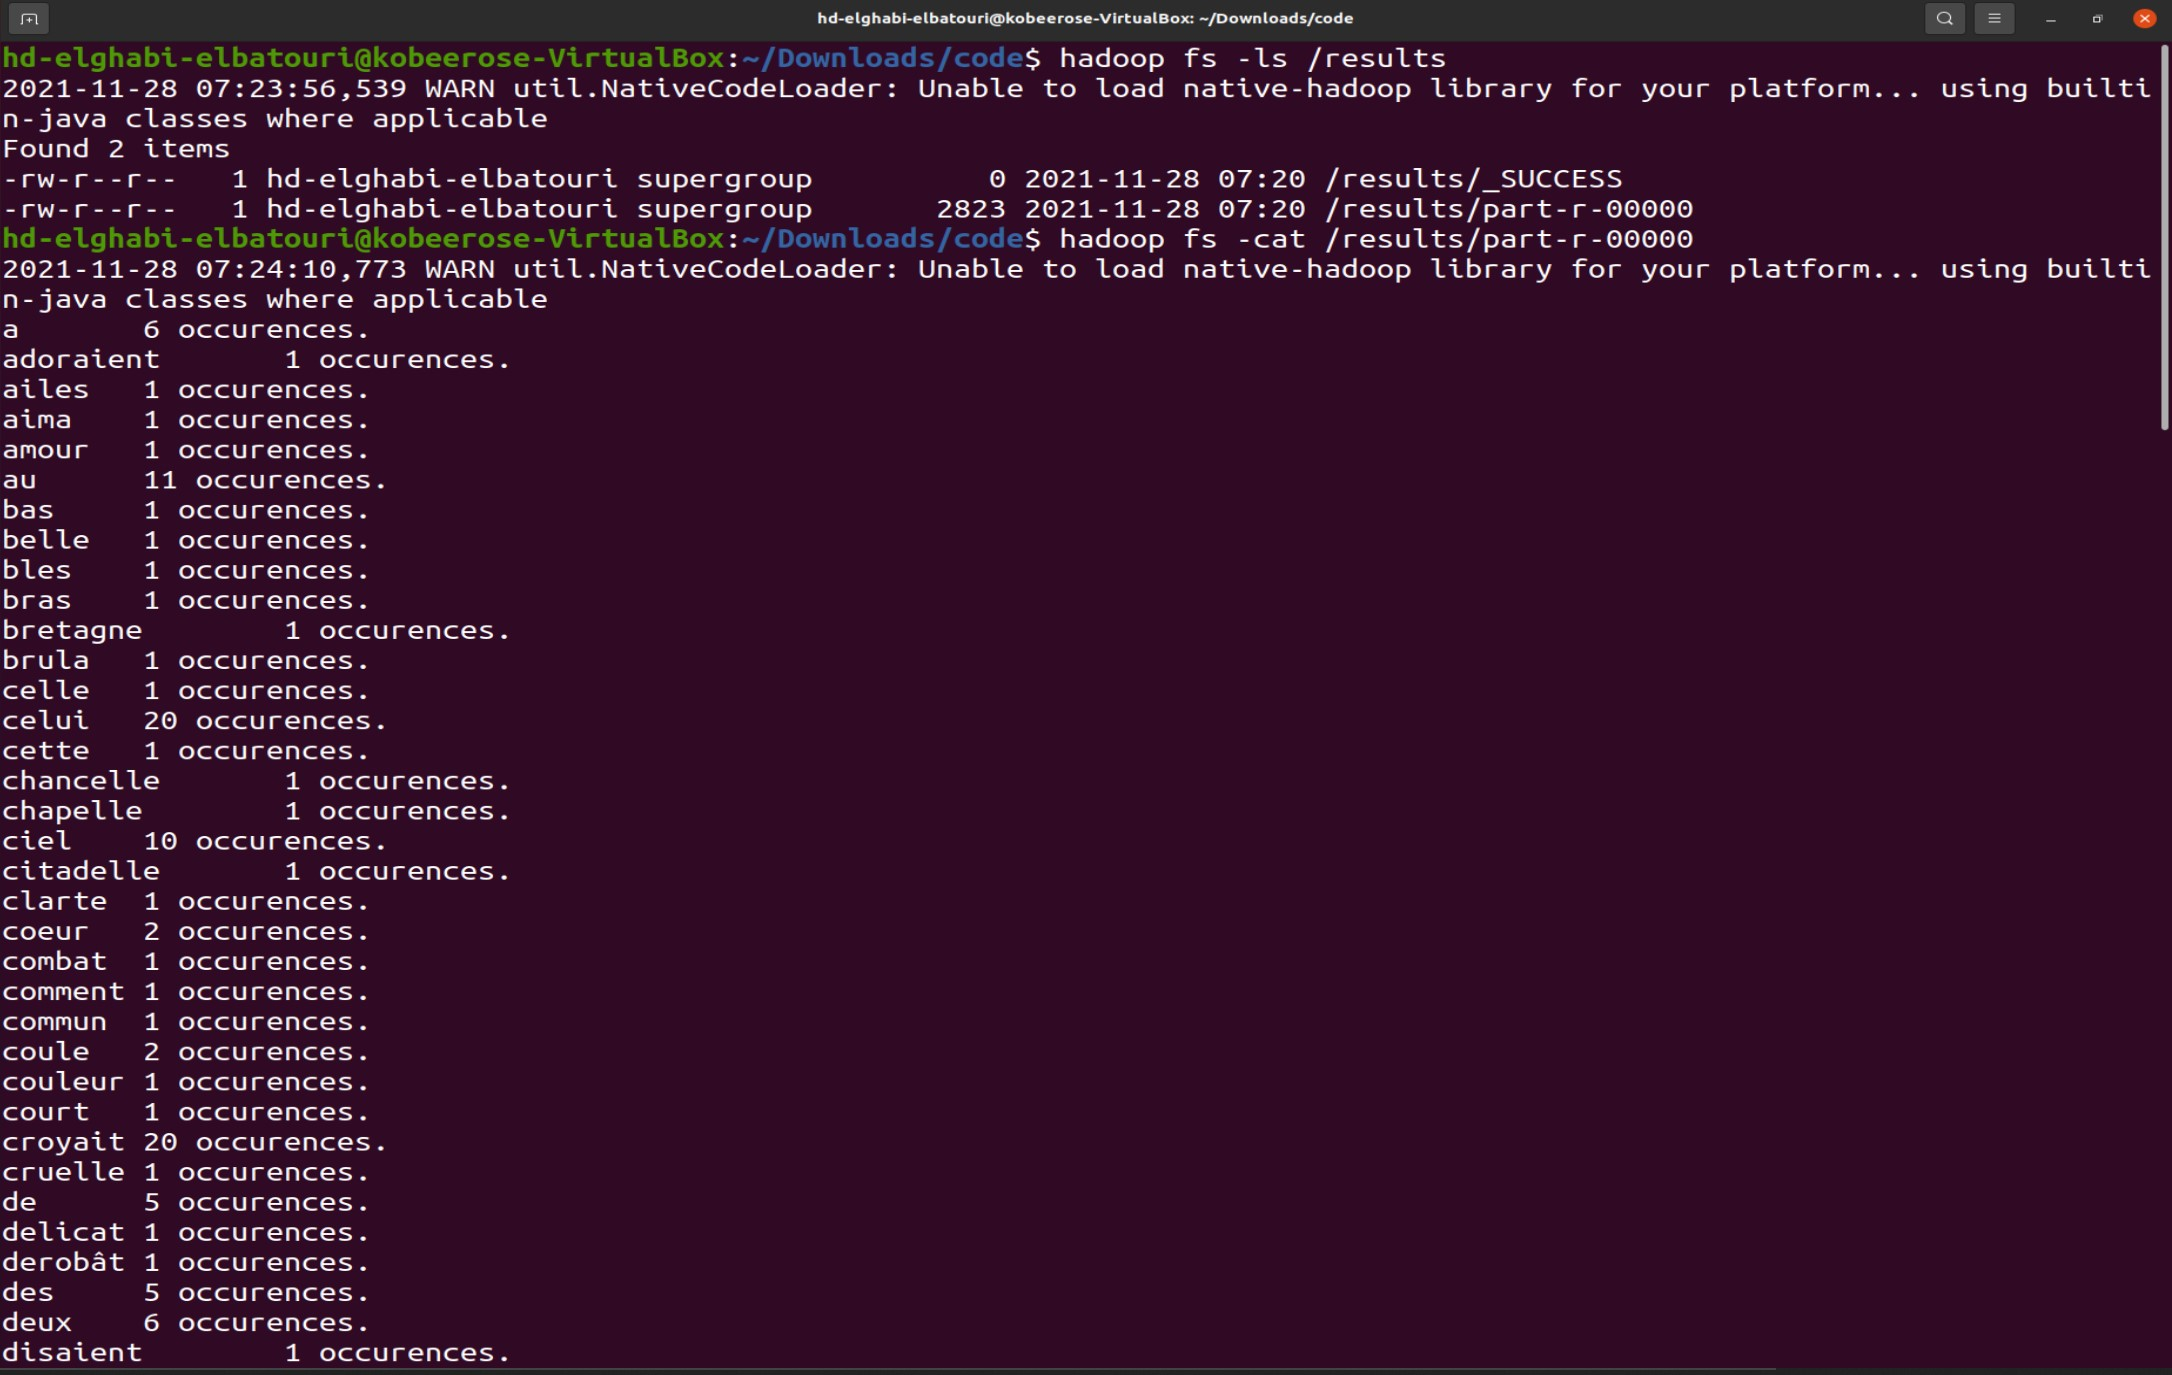
\includegraphics[width=1\linewidth]{Big_Data/Hadoop/1-Node Map_Reduce/Showing results} 
\end{center} 
\caption{Showing results} 
\end{figure} 
\FloatBarrier

\par We use stop-dfs.sh and stop-yarn.sh to stop all daemons running on our virtual machine
\\
\begin{figure}[!htb] 
\begin{center} 
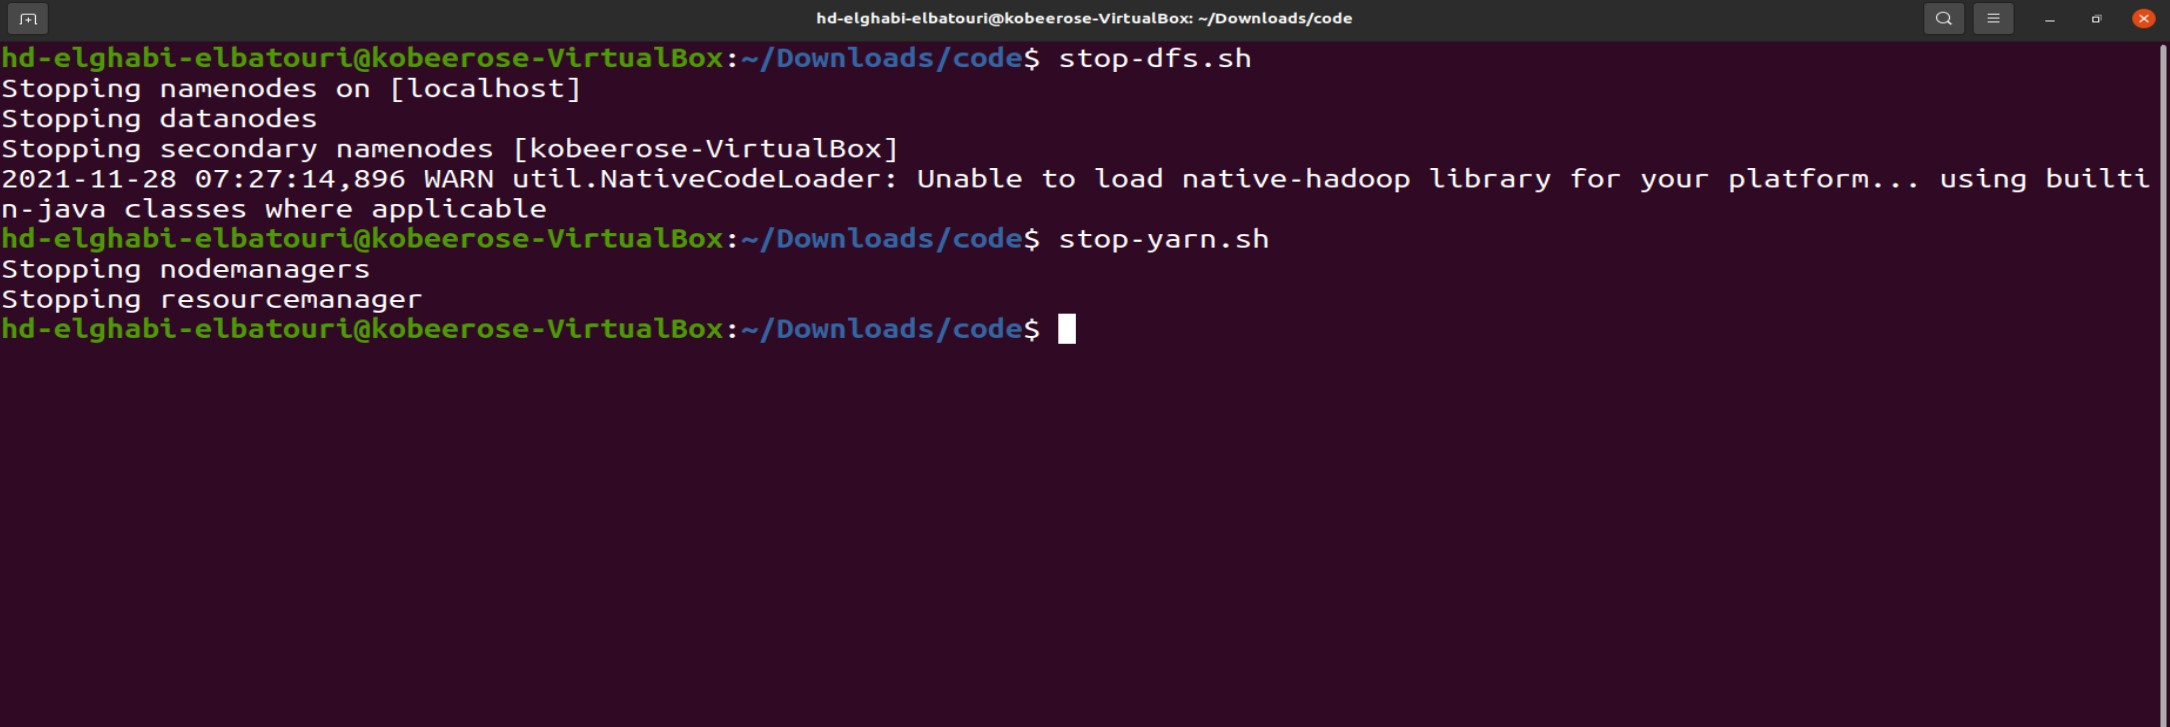
\includegraphics[width=1\linewidth]{Big_Data/Hadoop/1-Node Map_Reduce/Stopping Hadoop and Yarn} 
\end{center} 
\caption{Stopping Hadoop and Yarn} 
\end{figure} 
\FloatBarrier


\end{spacing}